\message{ !name(slides.tex)}% March 2012
% Autor: Mandy Vogel
% deducer

\documentclass[xcolor={table},c]{beamer}
% \usetheme[backgroundimagefile=mathe]{diepen}
\usetheme{Singapore}
\useoutertheme{miniframes}

%\setbeamerfont{block title}{size=\small,series=\bfseries}
%\setbeamerfont{block body}{size=\footnotesize}

% \usecolortheme{beetle}
\usepackage{linkimage}

\begin{document}

\message{ !name(slides.tex) !offset(-3) }


\title{Deducer}   
\author{Mandy Vogel} 
\date{\today}

\AtBeginSection{
  \begin{frame}<beamer>{Table of Contents}
    \tableofcontents[currentsection]
  \end{frame}}

\begin{frame}
\titlepage
\end{frame}

\begin{frame}{Table of Contents}
\frametitle{Table of Contents}\tableofcontents
\end{frame}

\begin{frame}\frametitle{Why Deducer ?}
Deducer is designed to be a free easy-to-use alternative to proprietary data analysis software such as SPSS, JMP, and Minitab. It has a menu system to perform common data manipulation and analysis tasks, and an excel-like spreadsheet in which to view and edit data frames. The goal of the project is two fold.
\begin{itemize}
\item Provide an intuitive graphical user interface (GUI) for R, encouraging non-technical users to learn and perform analyses without programming getting in their way.
\item   Increase the efficiency of expert R users when performing common tasks by replacing hundreds of keystrokes with a few mouse clicks. Also, as much as possible the GUI should not get in their way if they just want to do some programming. 
  \end{itemize}
\end{frame}

\section{Ready to Use}
\subsection{Run Deducer}
\begin{frame}{Run}
  \begin{itemize}
    \item from within R:
      \begin{itemize}
        \item run R
        \item type \texttt{library(JGR)}
        \item followed by \texttt{JGR()}
      \end{itemize}
    \item there is also a script created during the installation; the path is shown when you start Deducer via R (e.g. \texttt{~/R/i686-pc-linux-gnu-library/2.14/JGR/scripts/run}
  \end{itemize}
\end{frame}

\subsection{Load and Install Packages}
\begin{frame}[allowframebreaks]\frametitle{Load Packages}
\begin{center}
\linkimage{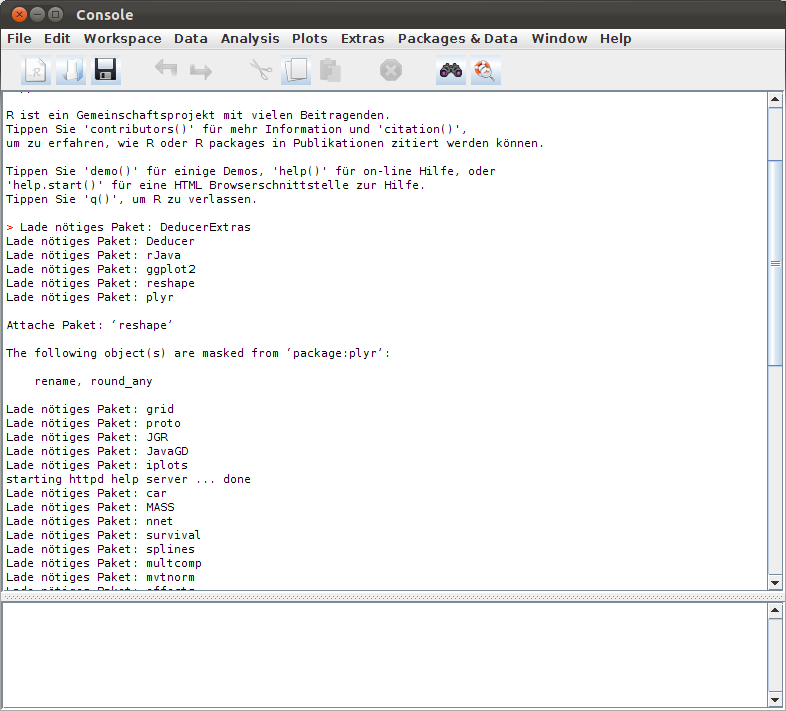
\includegraphics[height=7cm]{whole.png}}{whole.png}\\
choose \texttt{Package Manager} from menu \texttt{Packages \& Data}
  
\includegraphics[width=11cm]{menupack1.png}\\
\vspace*{0.5cm}
  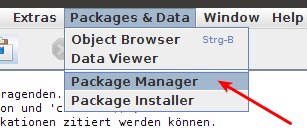
\includegraphics[width=7cm]{menupack2.png}
\end{center}
\end{frame}

\begin{frame}[shrink=5]{Package Manager}
    \vspace*{0.5cm}
\begin{columns}[c]
  \begin{column}{0.5\textwidth}
  \linkimage{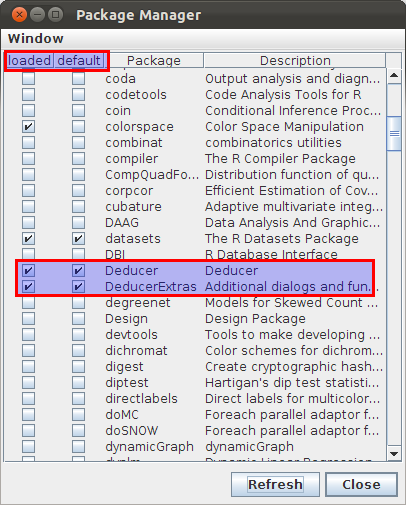
\includegraphics[width=5.5cm]{packman1.png}}{packman1.png}
  \end{column}
  \begin{column}{0.5\textwidth}Now you can choose the packages you want to load for the current session and those you want to load by default each time. 

The packages \texttt{Deducer} and \texttt{DeducerExtra} should be chosen as default.
  \end{column}
 \end{columns}
\end{frame}

\begin{frame}\frametitle{Package Installer}
  \begin{columns}
    \begin{column}{0.3\textwidth}
      \linkimage{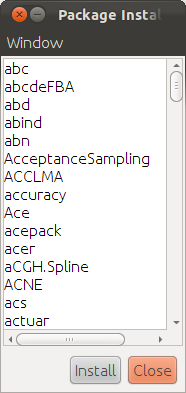
\includegraphics[height=7cm]{packinst1.png}}{packinst1.png}
    \end{column}
    \begin{column}{0.7\textwidth}
      The package installer can also be found in the menu \texttt{Packages \& Data}
    \end{column}
  \end{columns}
\end{frame}

\begin{frame}[fragile]\frametitle{Additional Deducer Packages}
  R-Forge offers a central platform for the development of R packages, R-related software and further projects. 
  There are three additional packages for Deducer. You can install them by typing:
% \begin{block}
\begin{semiverbatim}
install.packages(c("DeducerRichOutput",
                   "DeducerANOVA",
                   "DeducerPSY220"),
                 repos="http://R-Forge.R-Project.org")
\end{semiverbatim}    
% \end{block}
\end{frame}

\begin{frame}[shrink=15]\frametitle{DeducerRichOutput}
\setbeamercolor{bfarb}{fg=blue,bg=blue!20}
\setbeamercolor{bfarb2}{fg=white,bg=blue!30}
\begin{beamercolorbox}[sep=0.5em,wd=14cm]{bfarb}
without DeducerRichOutput\\
\linkimage{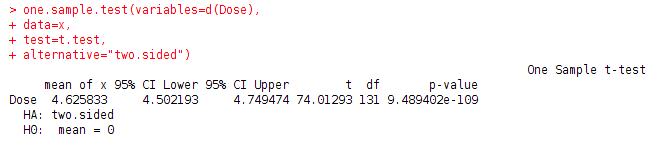
\includegraphics[width=9cm]{outputnormal.png}}{outputnormal.png}\\
\end{beamercolorbox}
\vspace*{0.4cm}
\begin{beamercolorbox}[sep=0.5em,wd=14cm]{bfarb}
with DeducerRichOutput\\
\linkimage{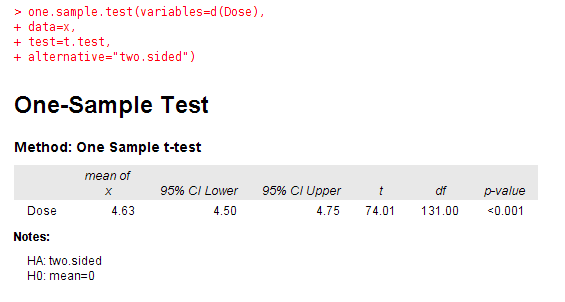
\includegraphics[width=9cm]{outputrich.png}}{outputrich.png}\\
\end{beamercolorbox}
\end{frame}

\section{Data}
\subsection{Loading Data}
\begin{frame}[shrink=5]\frametitle{data types Deducer can handle}
  The \texttt{load data} menu can handle the following data types
\begin{center}
    \rowcolors[]{1}{gray!10}{gray!30}
  \begin{tabular}{@{} >{\ttfamily}l l l} 
    \rowcolor{gray!40}
    File Type&Extension\\
    R workspace&*.rda and *.rdata\\
    R object&*.robj\\
    Comma seperated&*.csv\\
    Text file&*.txt\\
    SPSS&*.sav\\
    SAS export&*.xpt\\
    DBase&*.dbf\\
    Stata&*.dta\\
    Systat&*.sys and *.syd\\
    ARFF&*.arff\\
    Epiinfo&*.rec\\
    Minitab&*.mtp\\
    S data dump&*.s3 \\
    Excel&*.xls,*.xlsx\\
  \end{tabular}
\end{center}
\end{frame}

\begin{frame}\frametitle{Loading Data}
  It is pretty easy: via the menu \texttt{File} $\to$ \texttt{Open Data}
  \begin{center}
    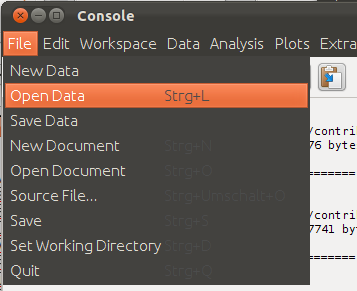
\includegraphics[width=5cm]{loaddata1.png} \hspace*{1cm}\linkimage{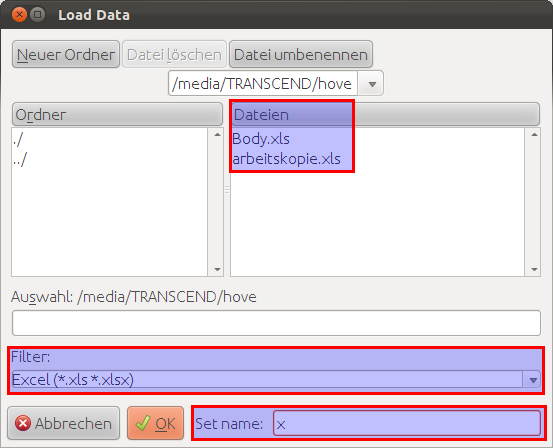
\includegraphics[width=5cm]{loaddata2.png}}{loaddata2.png}
  \end{center}
\end{frame}

 \subsection{Data Viewer}
 \begin{frame}\frametitle{Open the Data Viewer}
   \begin{columns}
     \begin{column}{0.5\textwidth}
   The data viewer provides an easy to use, spreadsheet-like environment to view and edit data. Copy and pasting is supported, and is compatible with Excel 2003\/2007, so data can be moved from Excel to R by simply copying it to the data viewer. Contextual menus are used to insert, delete and copy rows and columns.
 \end{column}
 \begin{column}{0.5\textwidth}
   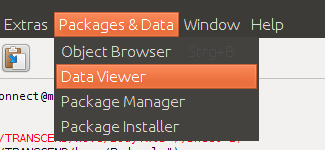
\includegraphics[width=5cm]{dataviewer1.png}
 \end{column}
 \end{columns}
 \end{frame}

\begin{frame}\frametitle{The Data Viewer - Data View}
  \begin{center}
    \linkimage{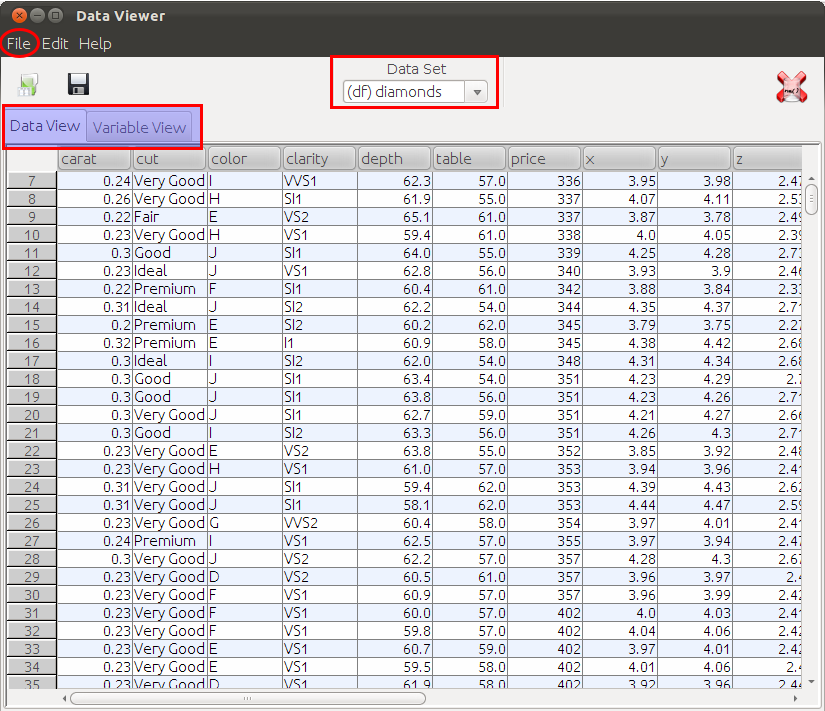
\includegraphics[height=7cm]{dataviewer2.png}}{dataviewer2.png}
  \end{center}
\end{frame}

\begin{frame}\frametitle{The Data Viewer - Data View 2}
  \begin{itemize}[<+->]
  \item a right click on the row or column headers 
    \begin{itemize}
    \item allows one to insert, copy and delete columns and rows \note{Add column sex}
    \item sort by one column
    \end{itemize}
  \item you can also edit the data
  \item in the drop down menu \texttt{Data Set} you can choose the data frame
  \end{itemize}
  \begin{center}
  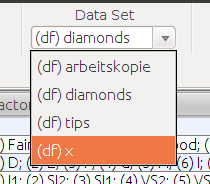
\includegraphics[width=4cm]{dataviewer4.png}
\end{center}
\end{frame}

\begin{frame}\frametitle{The Data Viewer - Variable View}
  \begin{center}
    \linkimage{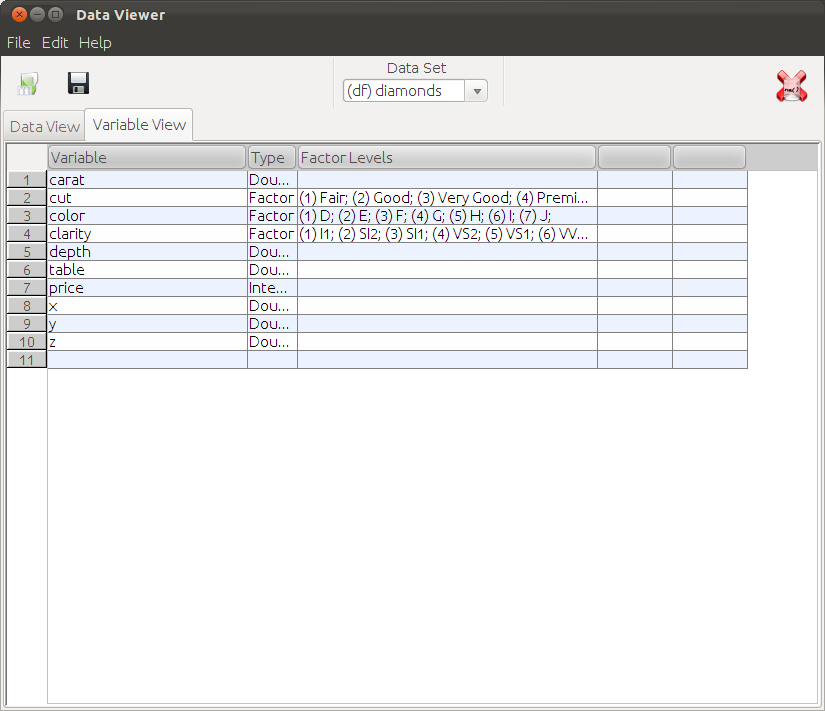
\includegraphics[height=7cm]{dataviewer3.png}}{dataviewer3.png}
  \end{center}
\end{frame}

\begin{frame}\frametitle{The Data Viewer - Variable View 2}
  In the variable view  The \texttt{variable} column represents the variable name. The \texttt{type} column determines the storage type.  
  \begin{itemize}
  \item the properties of each variable in the data frame can be edited
  \item the type column determines the storage type; variables can be stored as 
    \begin{itemize}
    \item Strings (character)
    \item Doubles (Numeric)
    \item Integers
    \item Logicals (yes/no) or 
    \item Factors
    \end{itemize}
  \item The levels of Factors are displayed in the 'Factor Levels' column, and can be edited by clicking on the appropriate cell, which brings up the Factor Editor
  \end{itemize}
\end{frame}

\begin{frame}\frametitle{The Data Viewer - Variable View 3}
\note{rename the sex variable, change it to factor, mention order, possibility to add levels, maybe contrasts}
The levels of Factors are displayed in the 'Factor Levels' column, and can be edited by clicking on the appropriate cell, which brings up the Factor Editor. 
\begin{center}
   \linkimage{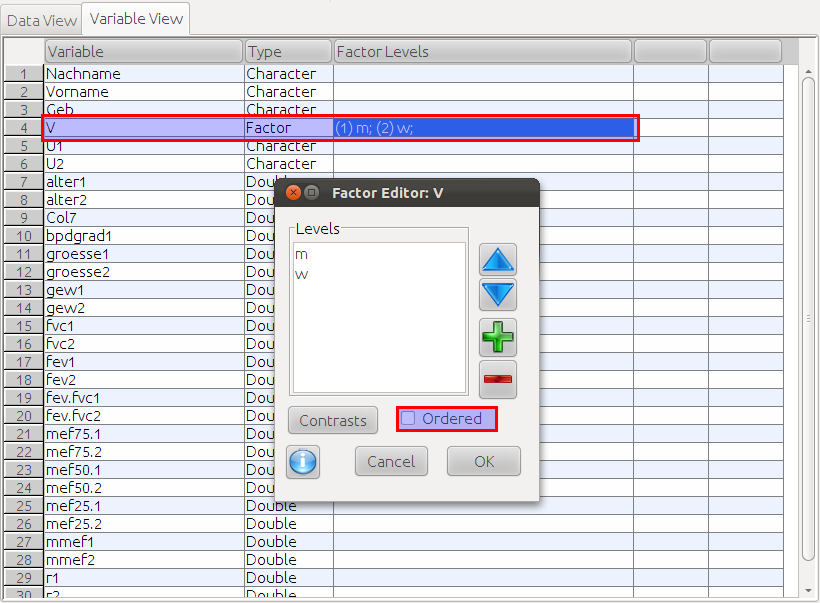
\includegraphics[height=5.5cm]{dataviewer5.png}}{dataviewer5.png}
\end{center}
\end{frame}

\section{Descriptive Statistics}
\subsection{Frequencies}
\begin{frame}\frametitle{Frequencies}
Frequency tables provide descriptive information for categorical and ordinal variables. They display the number of cases that fall into each category of a specific variable, as well as calculate percentages. 
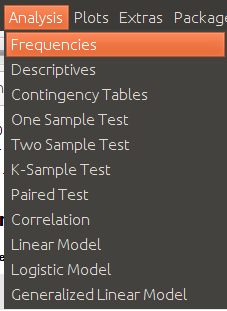
\includegraphics[width=3.5cm]{frequ1.png} \hspace*{1cm} 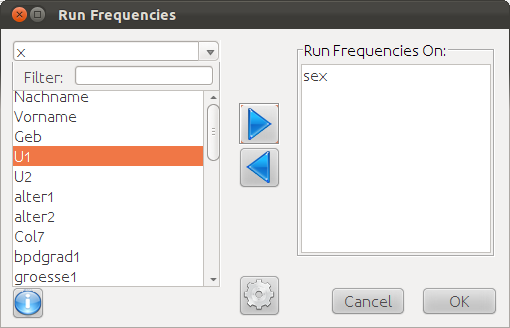
\includegraphics[width=5cm]{frequ2.png}
\end{frame}


\begin{frame}\frametitle{Frequencies Output}
\begin{columns}
\begin{column}{0.5\textwidth}
With DeducerRichOutput\\
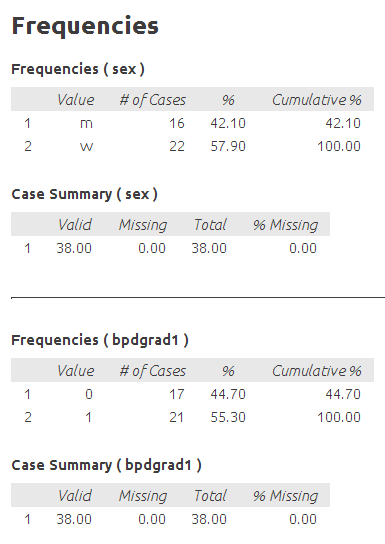
\includegraphics[height=7cm]{frequ3.png} 
\end{column}
\begin{column}{0.5\textwidth}
Without DeducerRichOutput\\
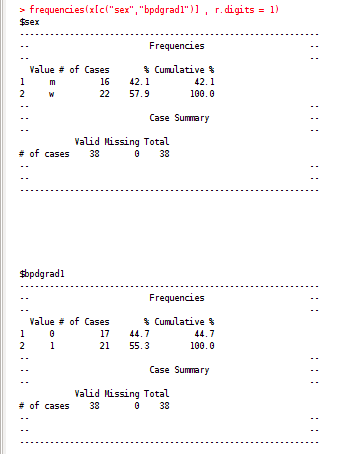
\includegraphics[height=7cm]{frequ4.png}
\end{column}
\end{columns}
\end{frame}

\subsection{Descriptives}
\begin{frame}\frametitle{Descriptives}
Calculates descriptive statistics for a set of variables. Possibly stratified by another set of variables. 
\begin{columns}
\begin{column}{0.5\textwidth}
\linkimage{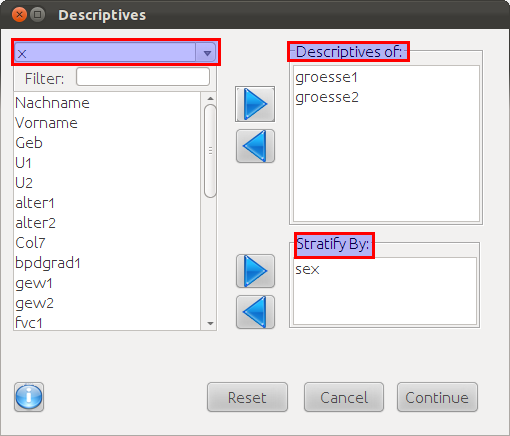
\includegraphics[width=5cm]{descr1.png}}{descr1.png}
\end{column}
\begin{column}{0.5\textwidth}
 \linkimage{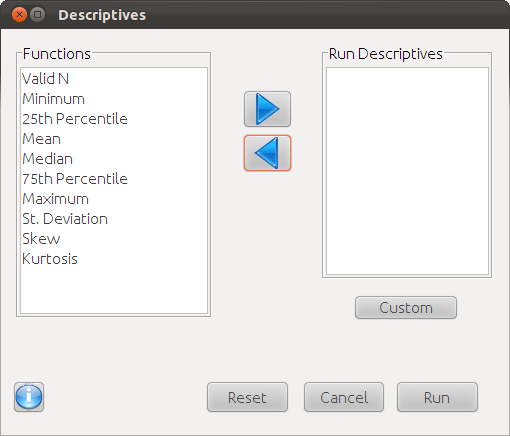
\includegraphics[width=5cm]{descr2.png}}{descr2.png}
\end{column}
\end{columns}
\end{frame}

\subsection{Contingency Tables}
\begin{frame}\frametitle{Contingency Tables}
Contingency tables (sometimes called crosstabs) are used to summarize and analyze the joint distribution of two variables, possibly stratified by a third. A table of observation counts will be created for each combination of the variables in the row list and each variable in the column list. If a stratum variable is specified, separate tables are created for each level of the variable. 
\begin{columns}
\begin{column}{0.4\textwidth}
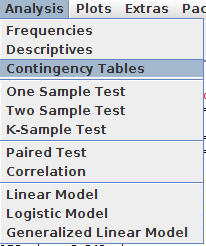
\includegraphics[width=3.2cm]{conting1.png}
\end{column}
\begin{column}{0.6\textwidth}
  \linkimage{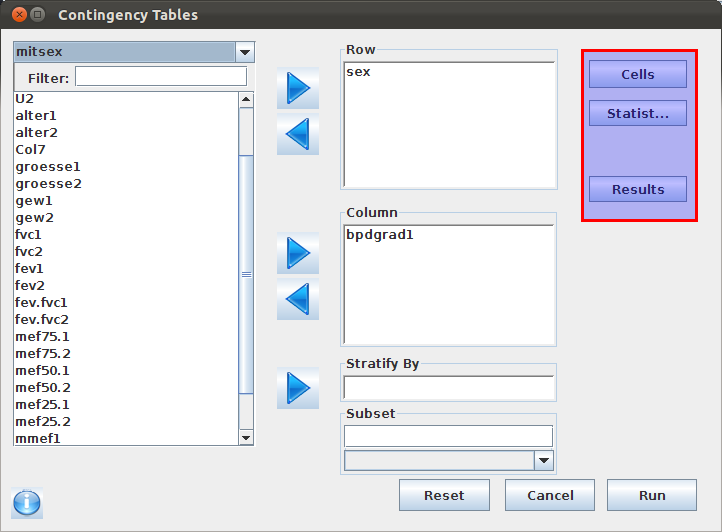
\includegraphics[width=5.5cm]{conting2.png}}{conting2.png}
\end{column}
\end{columns}
\end{frame}

\begin{frame}[shrink=5]\frametitle{Contingency Tables - Cells}
 In addition to observation counts, there are a number of additional cell values that can be displayed.
\begin{enumerate}[<+->]
\item Percentages
\begin{enumerate}
  \item Row - Percentage in cell out of observations within each row
  \item Column - Percentage in cell out of observations within each column
  \item Total - Percentage in cell 
\end{enumerate}
\item $\chi^2$-test
\begin{enumerate}[<+->]
\item Expected - The expected count of the cell if there were no relationship between the two variables
\item Residuals - The observed count minus the expected count.
\item Standardized residuals - The residuals standardized such that (if the two variables were independent) they have mean 0 and standard deviation 1. These residuals are useful in determining which cells of a contingency table contribute most to a significant $\chi^2$ test.
\item Adjusted residuals - These adjust the residuals by the row and column totals. 
\end{enumerate}
\end{enumerate}
\end{frame}

\begin{frame}\frametitle{Contingency Tables - Cells}
\begin{center}
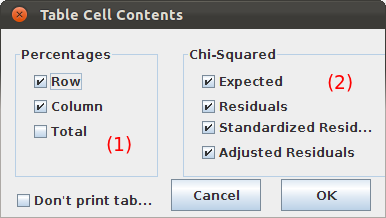
\includegraphics[width=6cm]{conting3.png}
\end{center}
\end{frame}

\begin{frame}\frametitle{Contingency Tables - Stats}
\begin{center}
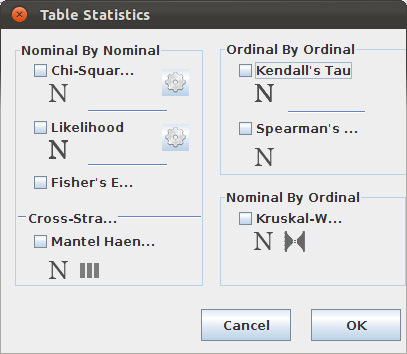
\includegraphics[width=7cm]{conting4.png}
\end{center}
\end{frame}

\begin{frame}\frametitle{Table Statistics - Nominal by Nominal}
  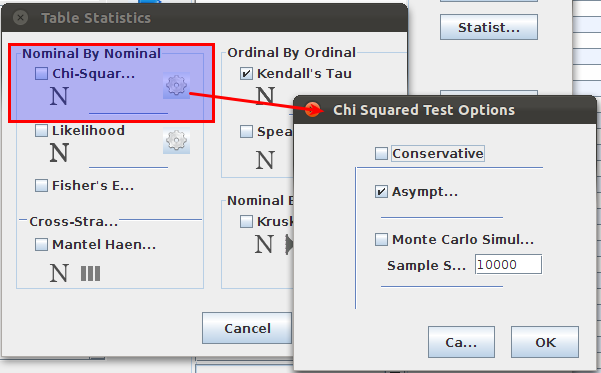
\includegraphics[width=8cm]{conting5.png}
\end{frame}


\note{Perhaps the most popular and pervasive method, the $\chi^2$ test can determine if there are any significant departures from independence. The $\chi^2$ test assumes the the cell counts are sufficiently large. Precisely what constitutes 'sufficiently large' is a mater of some debate. 

One rule of thumb is that all expected cell counts should be \emph{above 5}. If this is violated, or if one wishes to be safe, the p-value can be calculated via monte \emph{carlo method}. This yields an approximate p-value that is more accurate at small sample sizes, and can be made arbitrarily exact by increasing the simulation sample size. 

By default no Yates continuity 'correction' is used, and the mid p-value is used for the monte carlo simulation. These can be changed to their more conservative counterparts by selecting the 'Conservative' option. }

\begin{frame}\frametitle{Table Statistics - Nominal by Nominal}
\begin{alertblock}{$\chi^2$-Test}
\begin{itemize} 
   \item test for any significant departures from independence
   \item cell counts have to be sufficiently large (rule of thumb $>5$)
   \item monte carlo method provides more accurate $p$-values for small sample sizes
   \item by default no Yates continuity 'correction' is used
   \item by default mid p-value is used for the monte carlo simulation
\end{itemize}
\end{alertblock}
\end{frame}

\begin{frame}[shrink=5]\frametitle{Table Statistics - Nominal by Nominal}
\begin{alertblock}{Likelihood Ratio (G test)}
  \begin{itemize}
  \item alternative to the $\chi^2$ test
  \item assumes that the cell counts are sufficiently large\note{ Williams' continuity 'correction' can be used by selecting the Conservative option}
  \end{itemize}
\end{alertblock}
\begin{alertblock}{Fisher's Exact}
\begin{itemize}
\item  used with very small sample sizes and very sparse data\note{It is exact, in that it is based on the exact distribution of the data. Deducer gives the mid p-value version of this test, whereas many other software packages give a more conservative version}
\end{itemize}
\end{alertblock}
\begin{alertblock}{Mantel-Haenszel} 
\begin{itemize}
\item like the $\chi^2$ test except that it adjusts for the stratification of a third variable
\item assumes that the cell counts for a collapsed table \note{(i.e. one that ignores the stratification variable)} are sufficiently large 
\item assumes that the relationship between the two variables of interest is constant across strata. 
\end{itemize}
\end{alertblock}
\end{frame}

\begin{frame}[shrink=4.5]\frametitle{Table Statistics - Ordinal by Ordinal}
Ordinal variable have a natural order, such as building floor or height. 
\begin{alertblock}{Kendall's $\tau$}
\begin{itemize} 
   \item measure of association similar to Pearson's correlation, but valid for discrete variables
   \item assumes a sufficiently large sample size 
\end{itemize}
\end{alertblock}
\begin{alertblock}{Spearman's $\rho$}
\begin{itemize} 
   \item Spearman's rho is the result of calculating the Pearson's correlation on the rank transformed data
\end{itemize}
\end{alertblock}
Both correlations measure the strength of monotonic assosiation between the two variables on a scale similar to Pearson's Correlation. The relative virtues of two approaches have been debated, and some favor the use of Kendall's tau. 
\end{frame}

\begin{frame}\frametitle{Table Statistics - Nominal by Ordinal}
\begin{alertblock}{Kruskal-Wallis}
\begin{itemize} 
   \item determines whether the ordinal variable tends to be greater in some categories of the nominal variable as opposed to others
   \item assumes a sufficiently large $N$
   \item assumes exchangability, which is similar to an equal variance assumption
\end{itemize}
\end{alertblock}
\end{frame}

\subsection{Tests}
\begin{frame}[shrink=6.5]\frametitle{One Sample Test}
\begin{columns}
\begin{column}{0.5\textwidth}
\begin{alertblock}{t-test}\small
\begin{itemize}
\item tests whether the mean of a population is not equal to a specified value
\item requires that either the sample size be sufficiently large, or the variable be normally distributed
\end{itemize}
\note{'Sufficiently large' in this case is fairly small for most distributions), as convergence of the test statistic to normality occurs rapidly. If outliers are present, this can lead to misleading inferences, so pre-screening of the data is recommended. The options button (the gear) allows for the specification of the alternate hypothesis and the null hypothesis mean. }
\end{alertblock}
\begin{alertblock}{ Shapiro-Wilk}
\begin{itemize}
\item performs the test against normality
\item determines if there is enough evidence to conclude that a variable in not normally distributed
\end{itemize}
\end{alertblock}
\note{statistical advice: One common, though misguided technique is to pre-screen variables used in other parametric analyses using this test. For example, one might check the normality of the residuals of a regression as a diagnostic technique. Hypothesis testing is fundimentally the wrong tool to use. At small sample sizes normality hypothesis tests will be insignificant even in the presence of large deviations from normality due to lack of power. At large sample sizes, data that is nearly normal (nothing is ever exactly normal) will trigger a significant normality test because the test has the power to detect even the smallest deviations from normality. These are precisely the opposite types of miscategorizations that an analyst wishes to make. Most statistical tests are robust to large departures from normality provided the sample size is large enough. So normality matters most in the situations where you have no statistical power to detect it.

A better alternative to normality testing is to examine the histogram. Is it skewed or roughly symmetrical? Are its tails fat? If your sample is small and your variable is skewed you can try switching to non-parametric methods or transforming the variable so it looks more normal. Alternatively if you can program, you can run simulations to assess the procedure's sensitivity to departures from normality.}
\end{column}
\begin{column}{0.5\textwidth}
  \linkimage{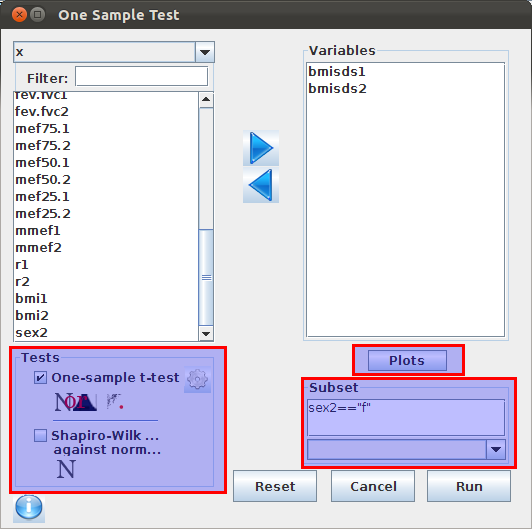
\includegraphics[width=5.5cm]{testonesample.png}}{testonesample.png}
\end{column}
\end{columns}
\end{frame}


\begin{frame}\frametitle{One Sample Test - Options}
\begin{columns}
\begin{column}{0.4\textwidth}
\begin{minipage}[c][4cm][c]{3.4cm}
\linkimage{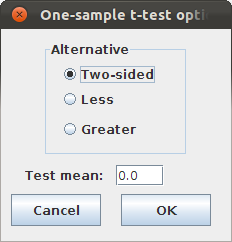
\includegraphics[width=3.2cm]{onesamplettestoptions.png}}{onesamplettestoptions.png}
\end{minipage}
\begin{minipage}[c][4cm][c]{3.4cm}
\linkimage{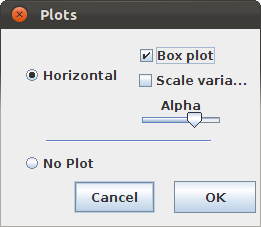
\includegraphics[width=3.2cm]{onesampleplot.png}}{onesampleplot.png}
\end{minipage}
\end{column}
\begin{column}{0.6\textwidth}
\begin{minipage}[c][4cm][c]{6cm}

\end{minipage}
\begin{minipage}[c][4cm][c]{6cm}

\end{minipage}
\end{column}
\end{columns} 
\end{frame}

\begin{frame}\frametitle{Two Sample Test}
\begin{columns}
\begin{column}{0.4\textwidth}
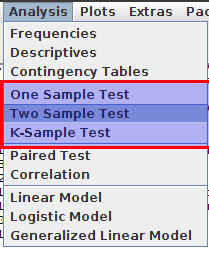
\includegraphics[width=3.2cm]{test1.png}
\end{column}
\begin{column}{0.6\textwidth}
  \linkimage{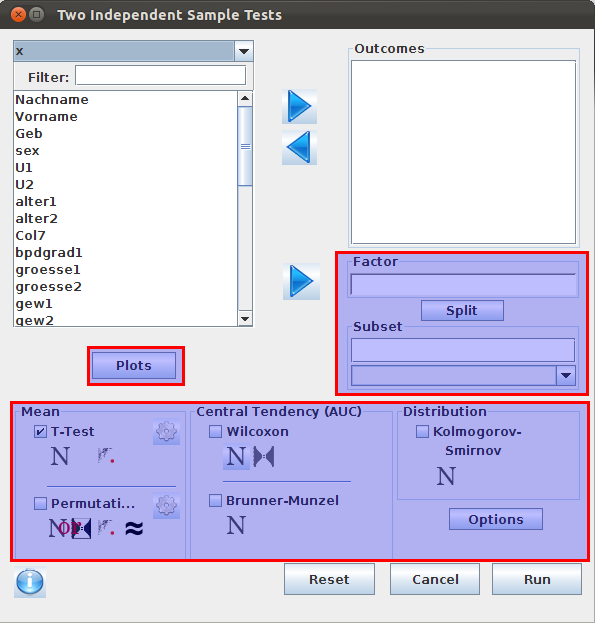
\includegraphics[width=5.5cm]{testtwosample.png}}{testtwosample.png}
\end{column}
\end{columns} 
\end{frame}


\begin{frame}\frametitle{K-Sample Test}
\begin{columns}
\begin{column}{0.4\textwidth}
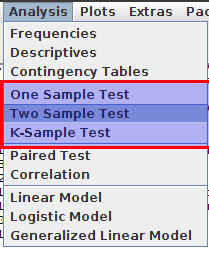
\includegraphics[width=3.2cm]{test1.png}
\end{column}
\begin{column}{0.6\textwidth}
  \linkimage{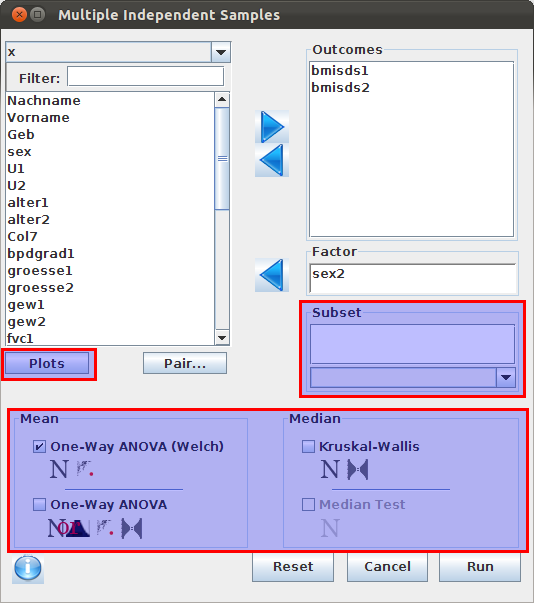
\includegraphics[width=5.5cm]{testmultsample.png}}{testmultsample.png}
\end{column}
\end{columns}
\end{frame}


\section{Full Screen}
%\flushlinkimages

\end{document}
\message{ !name(slides.tex) !offset(-444) }
